\chapter{Literature Review}
\label{chap::literature_review}

This is the section describing the related work and outlining the research gap that your document is addressing.

This is an example of an ``in-text'' citation: \cite{jordan2015machine}.

Remember to insert each entry to the \textit{references.bib} file.

\textbf{Do not} describe concepts that have limited connection to your goal. Whoever is going to read this thesis is meant to be an ``expert''!

Use schemas or figures if necessary: they help a lot in understanding. If you take the schemas from previous work, do cite them in the caption. Figures can be cited with \textbackslash ref command such as Figure \ref{fig::example_picture}.

\begin{figure}[!htbp]
    \centering
    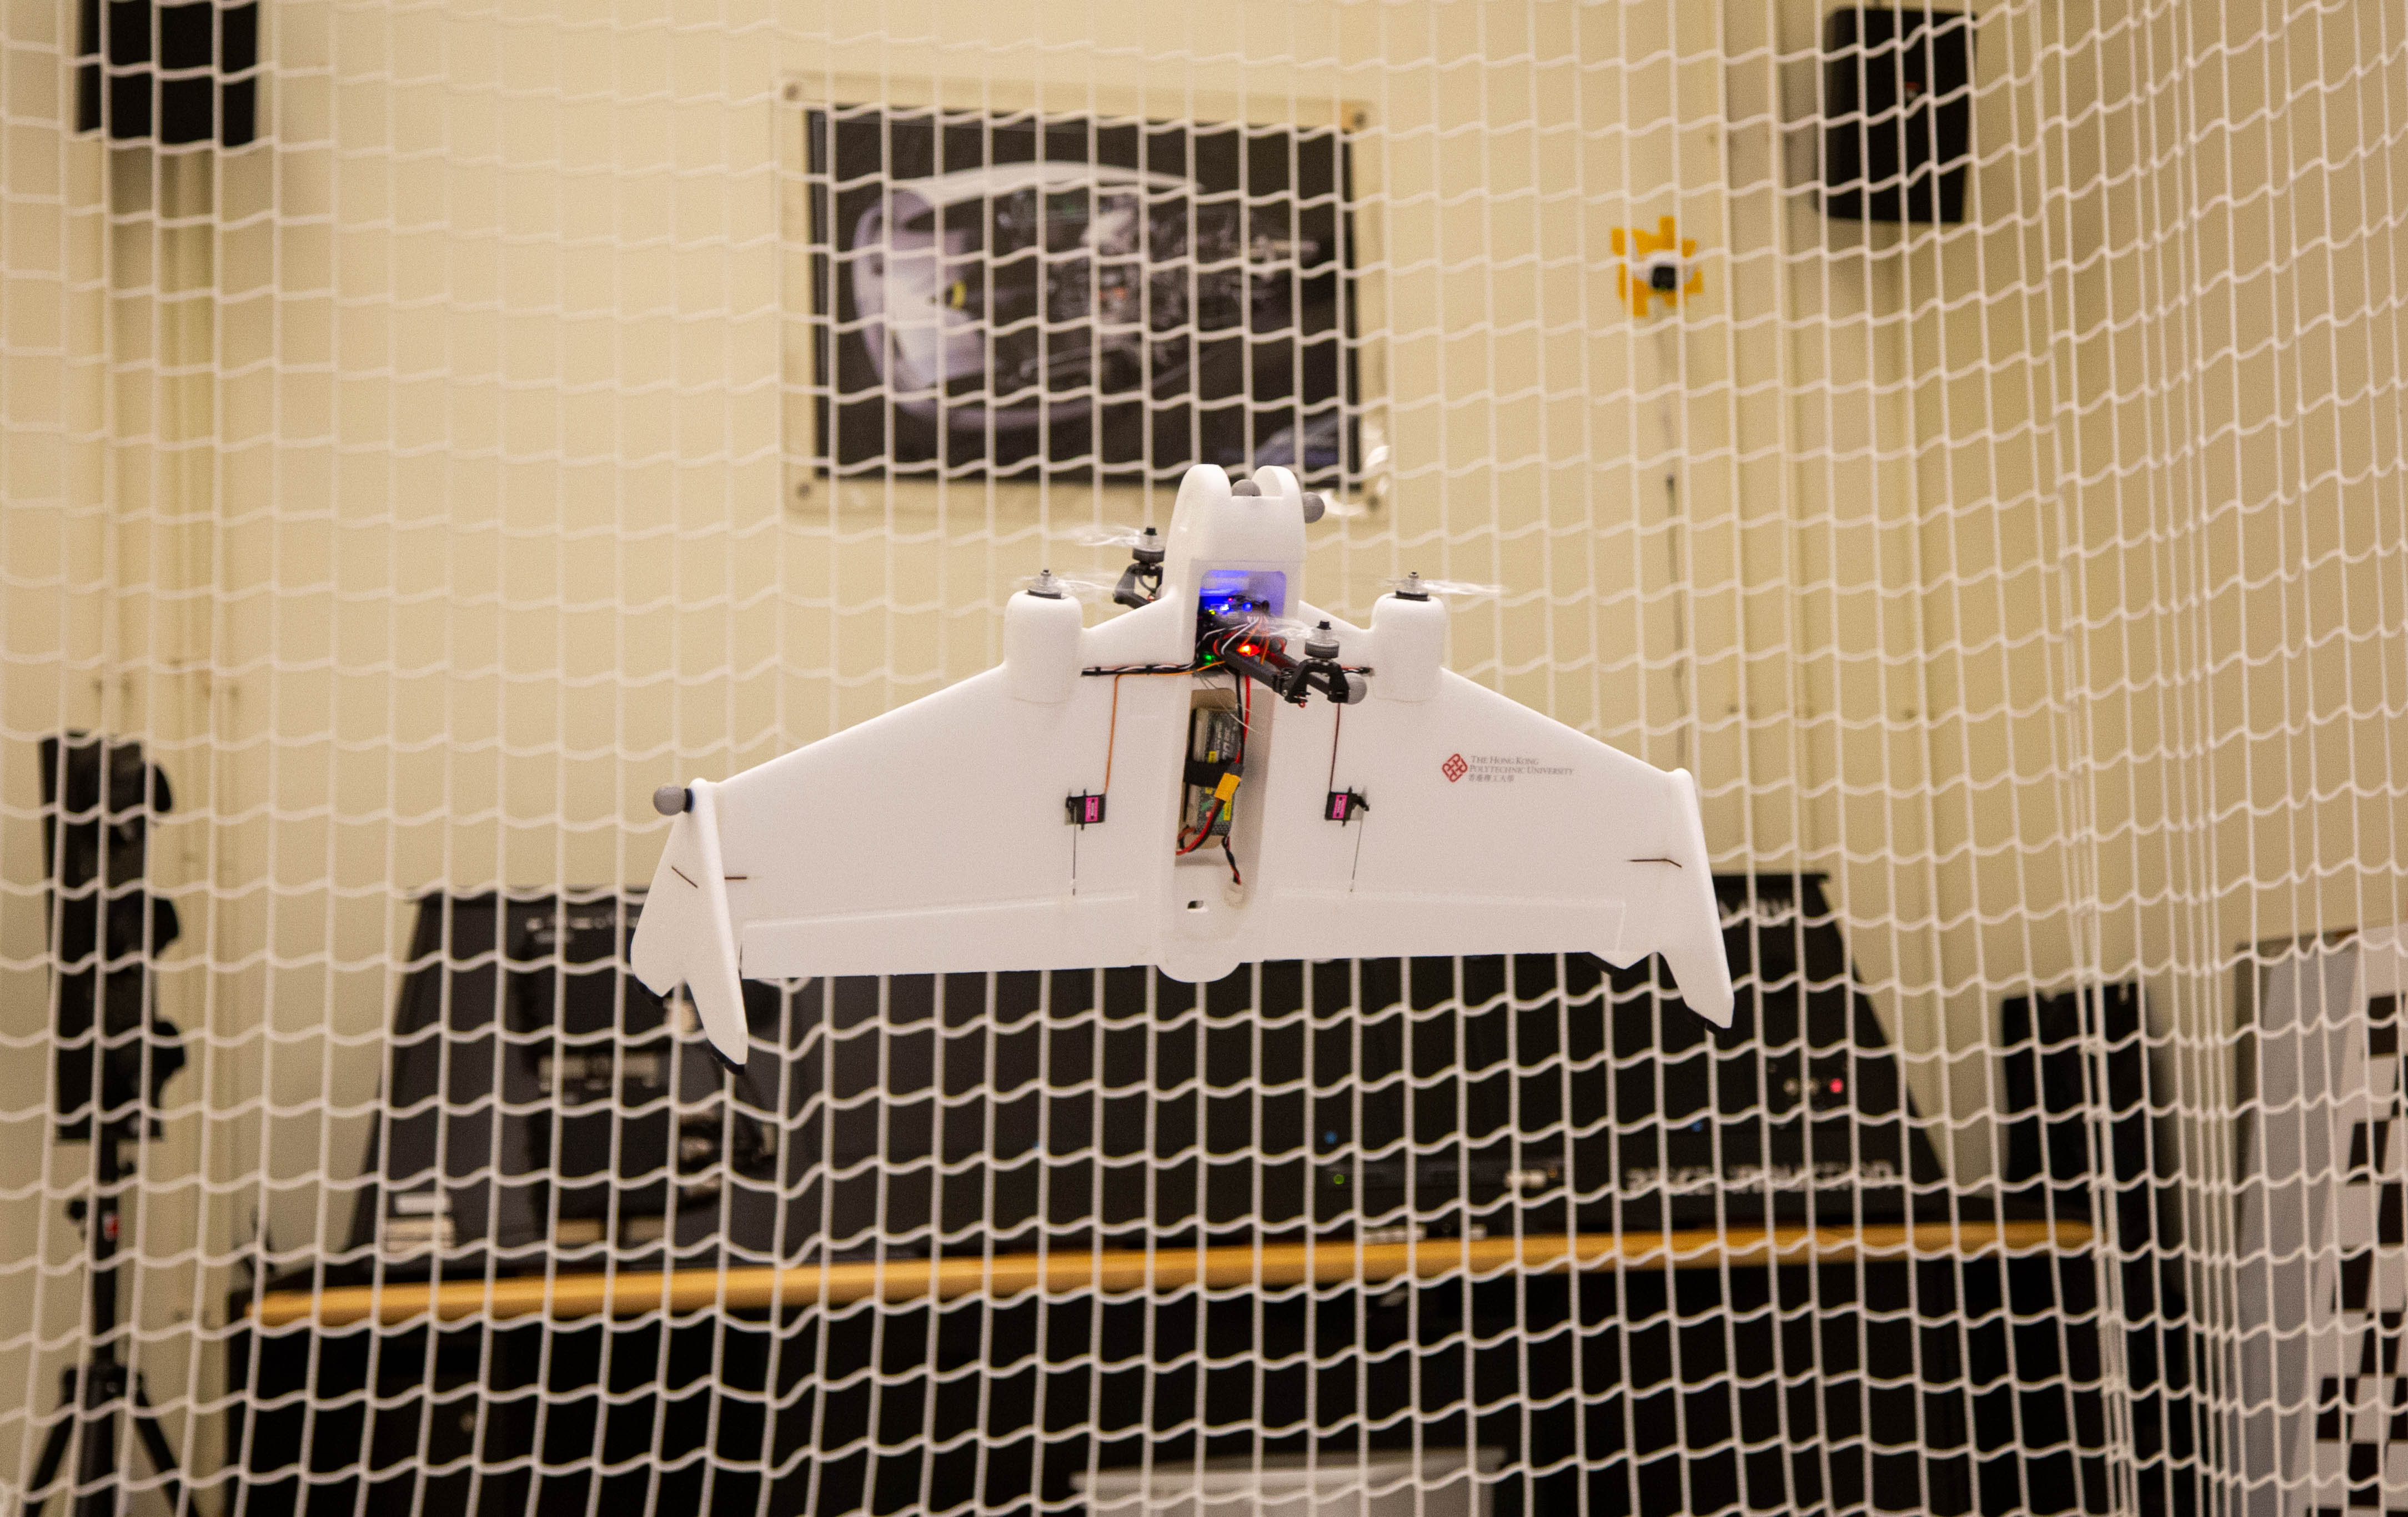
\includegraphics[width=0.75\columnwidth]{images/figures/example_figure.jpg}
    \caption{The caption of figures goes BELOW the figure.}
    \label{fig::example_picture}
\end{figure}

To include subfigures follow the following example:

\begin{figure}[!htbp]
    \begin{subfigure}{\textwidth}
        \centering
        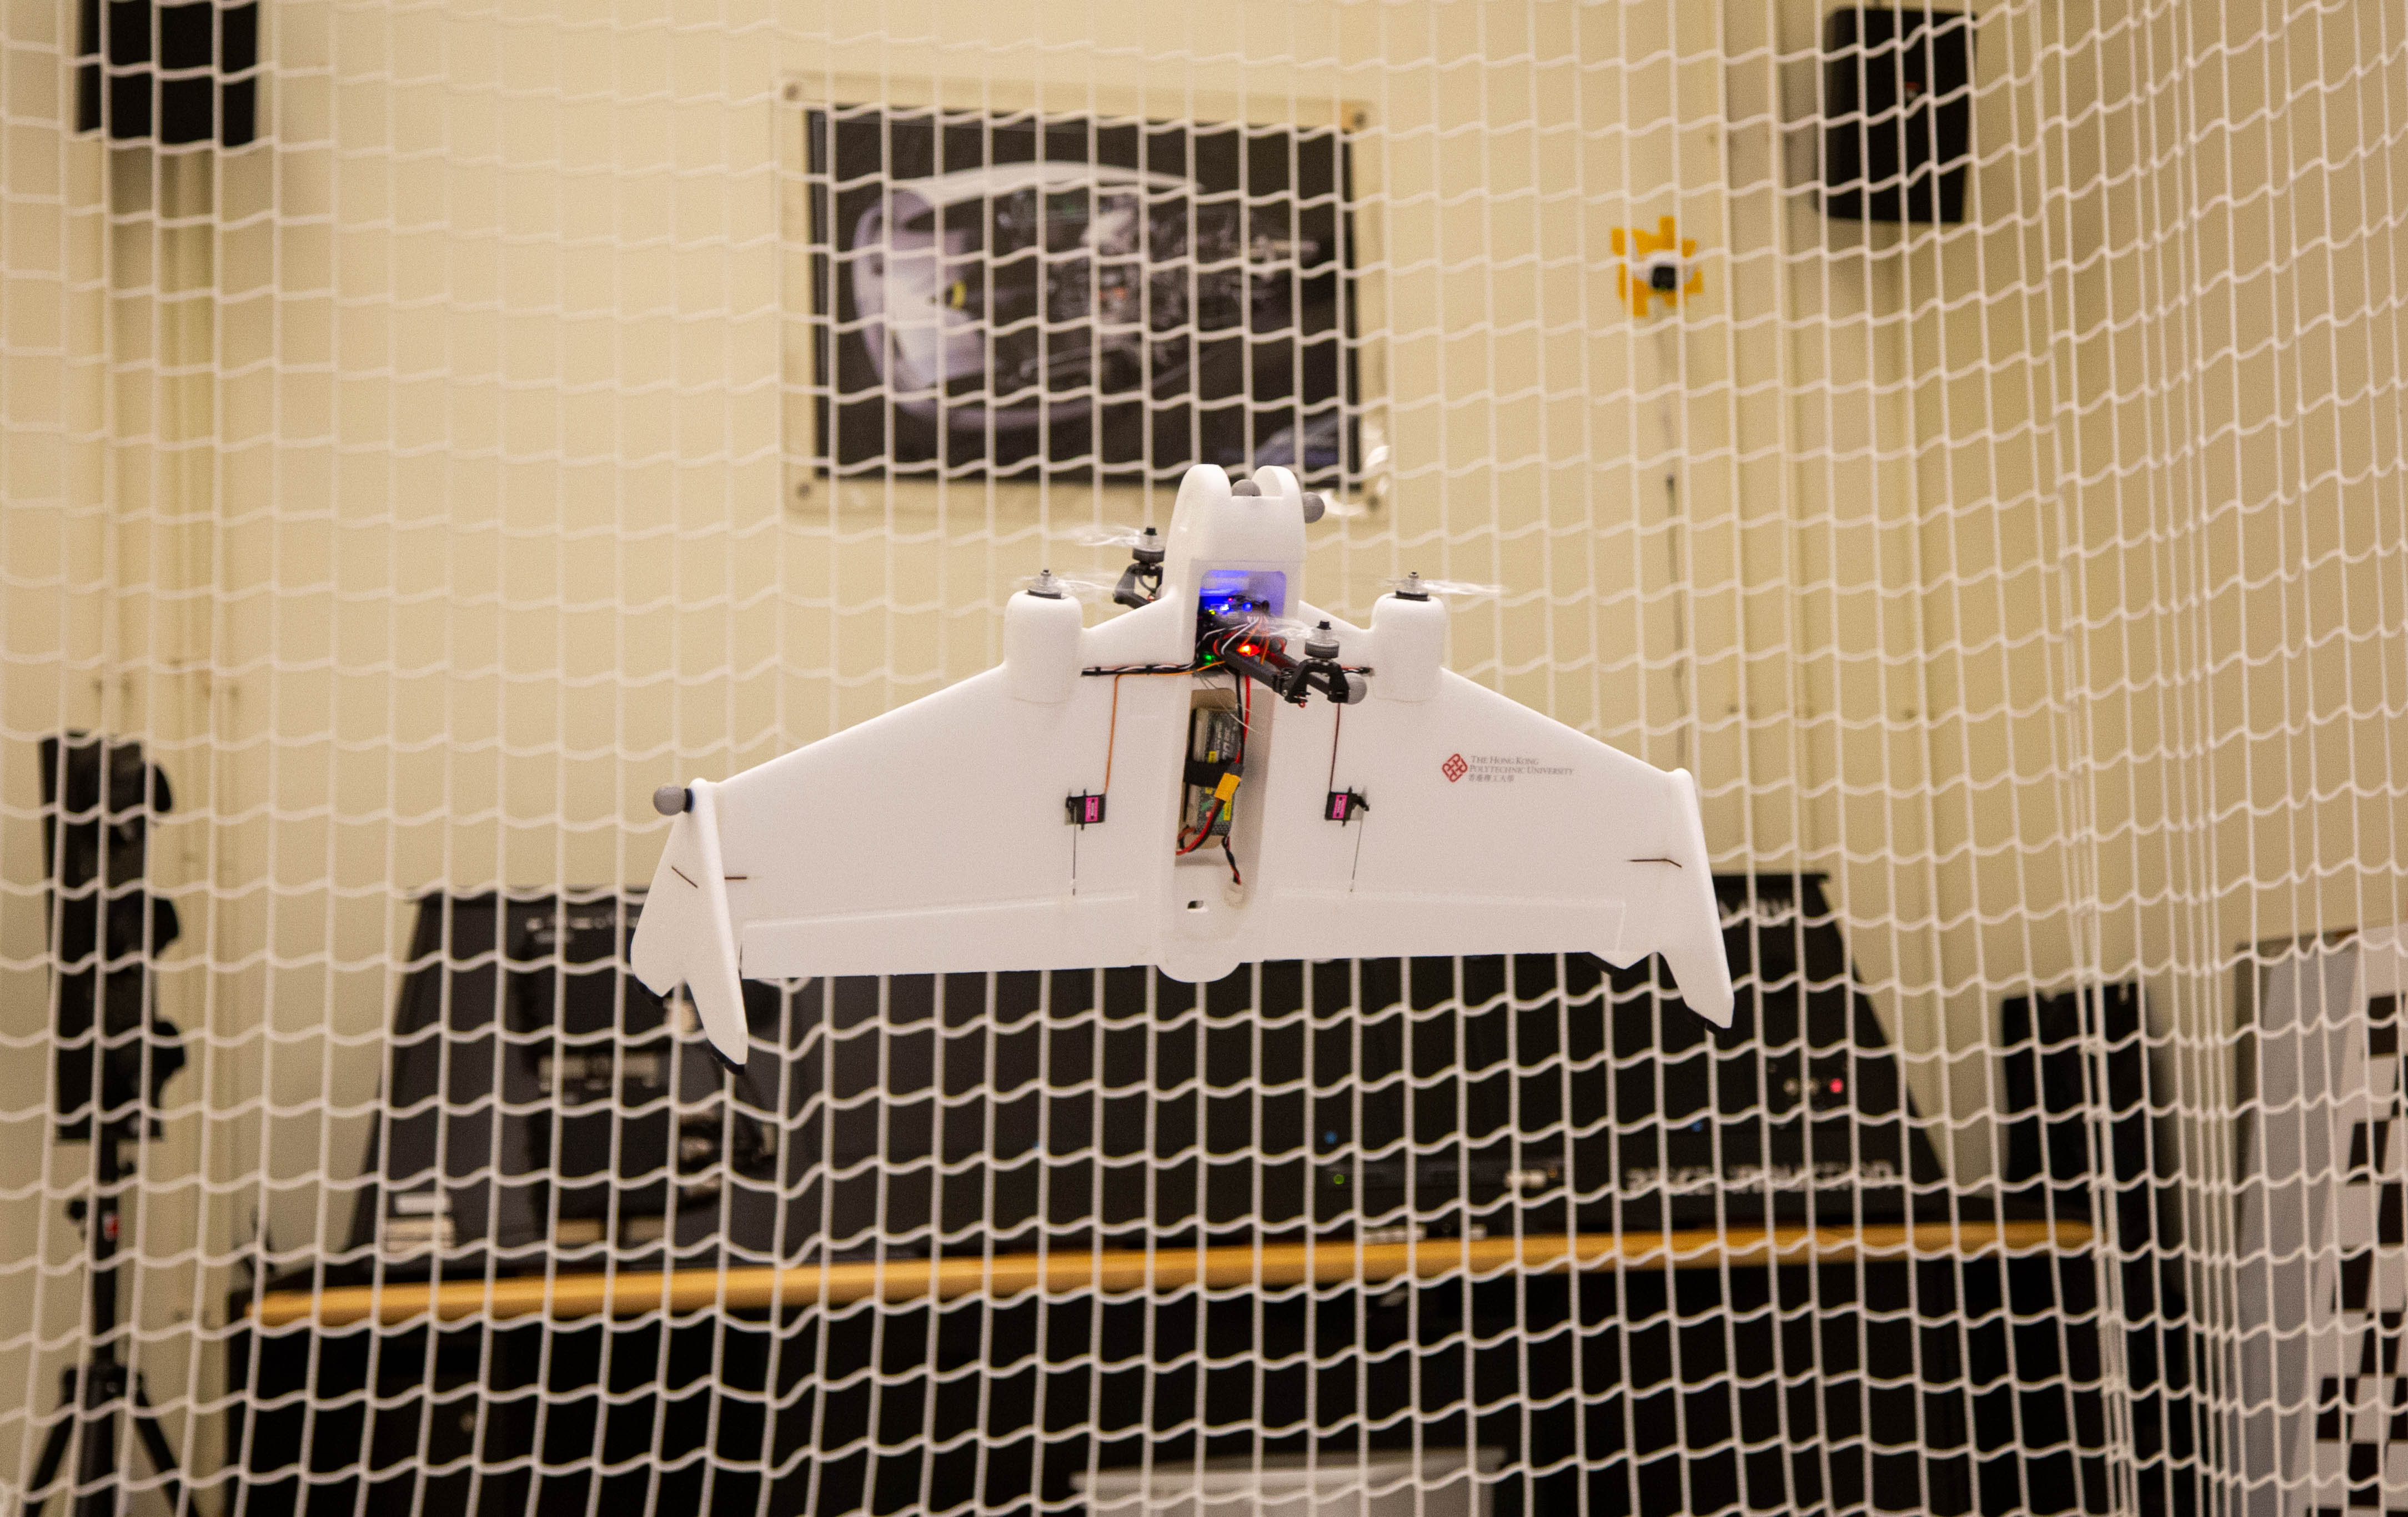
\includegraphics[width=0.7\textwidth]{images/figures/example_figure.jpg}
        \caption{Subfigure a.}
        \label{fig::subfigure_a}
    \end{subfigure}
    \begin{subfigure}{\textwidth}
        \centering
	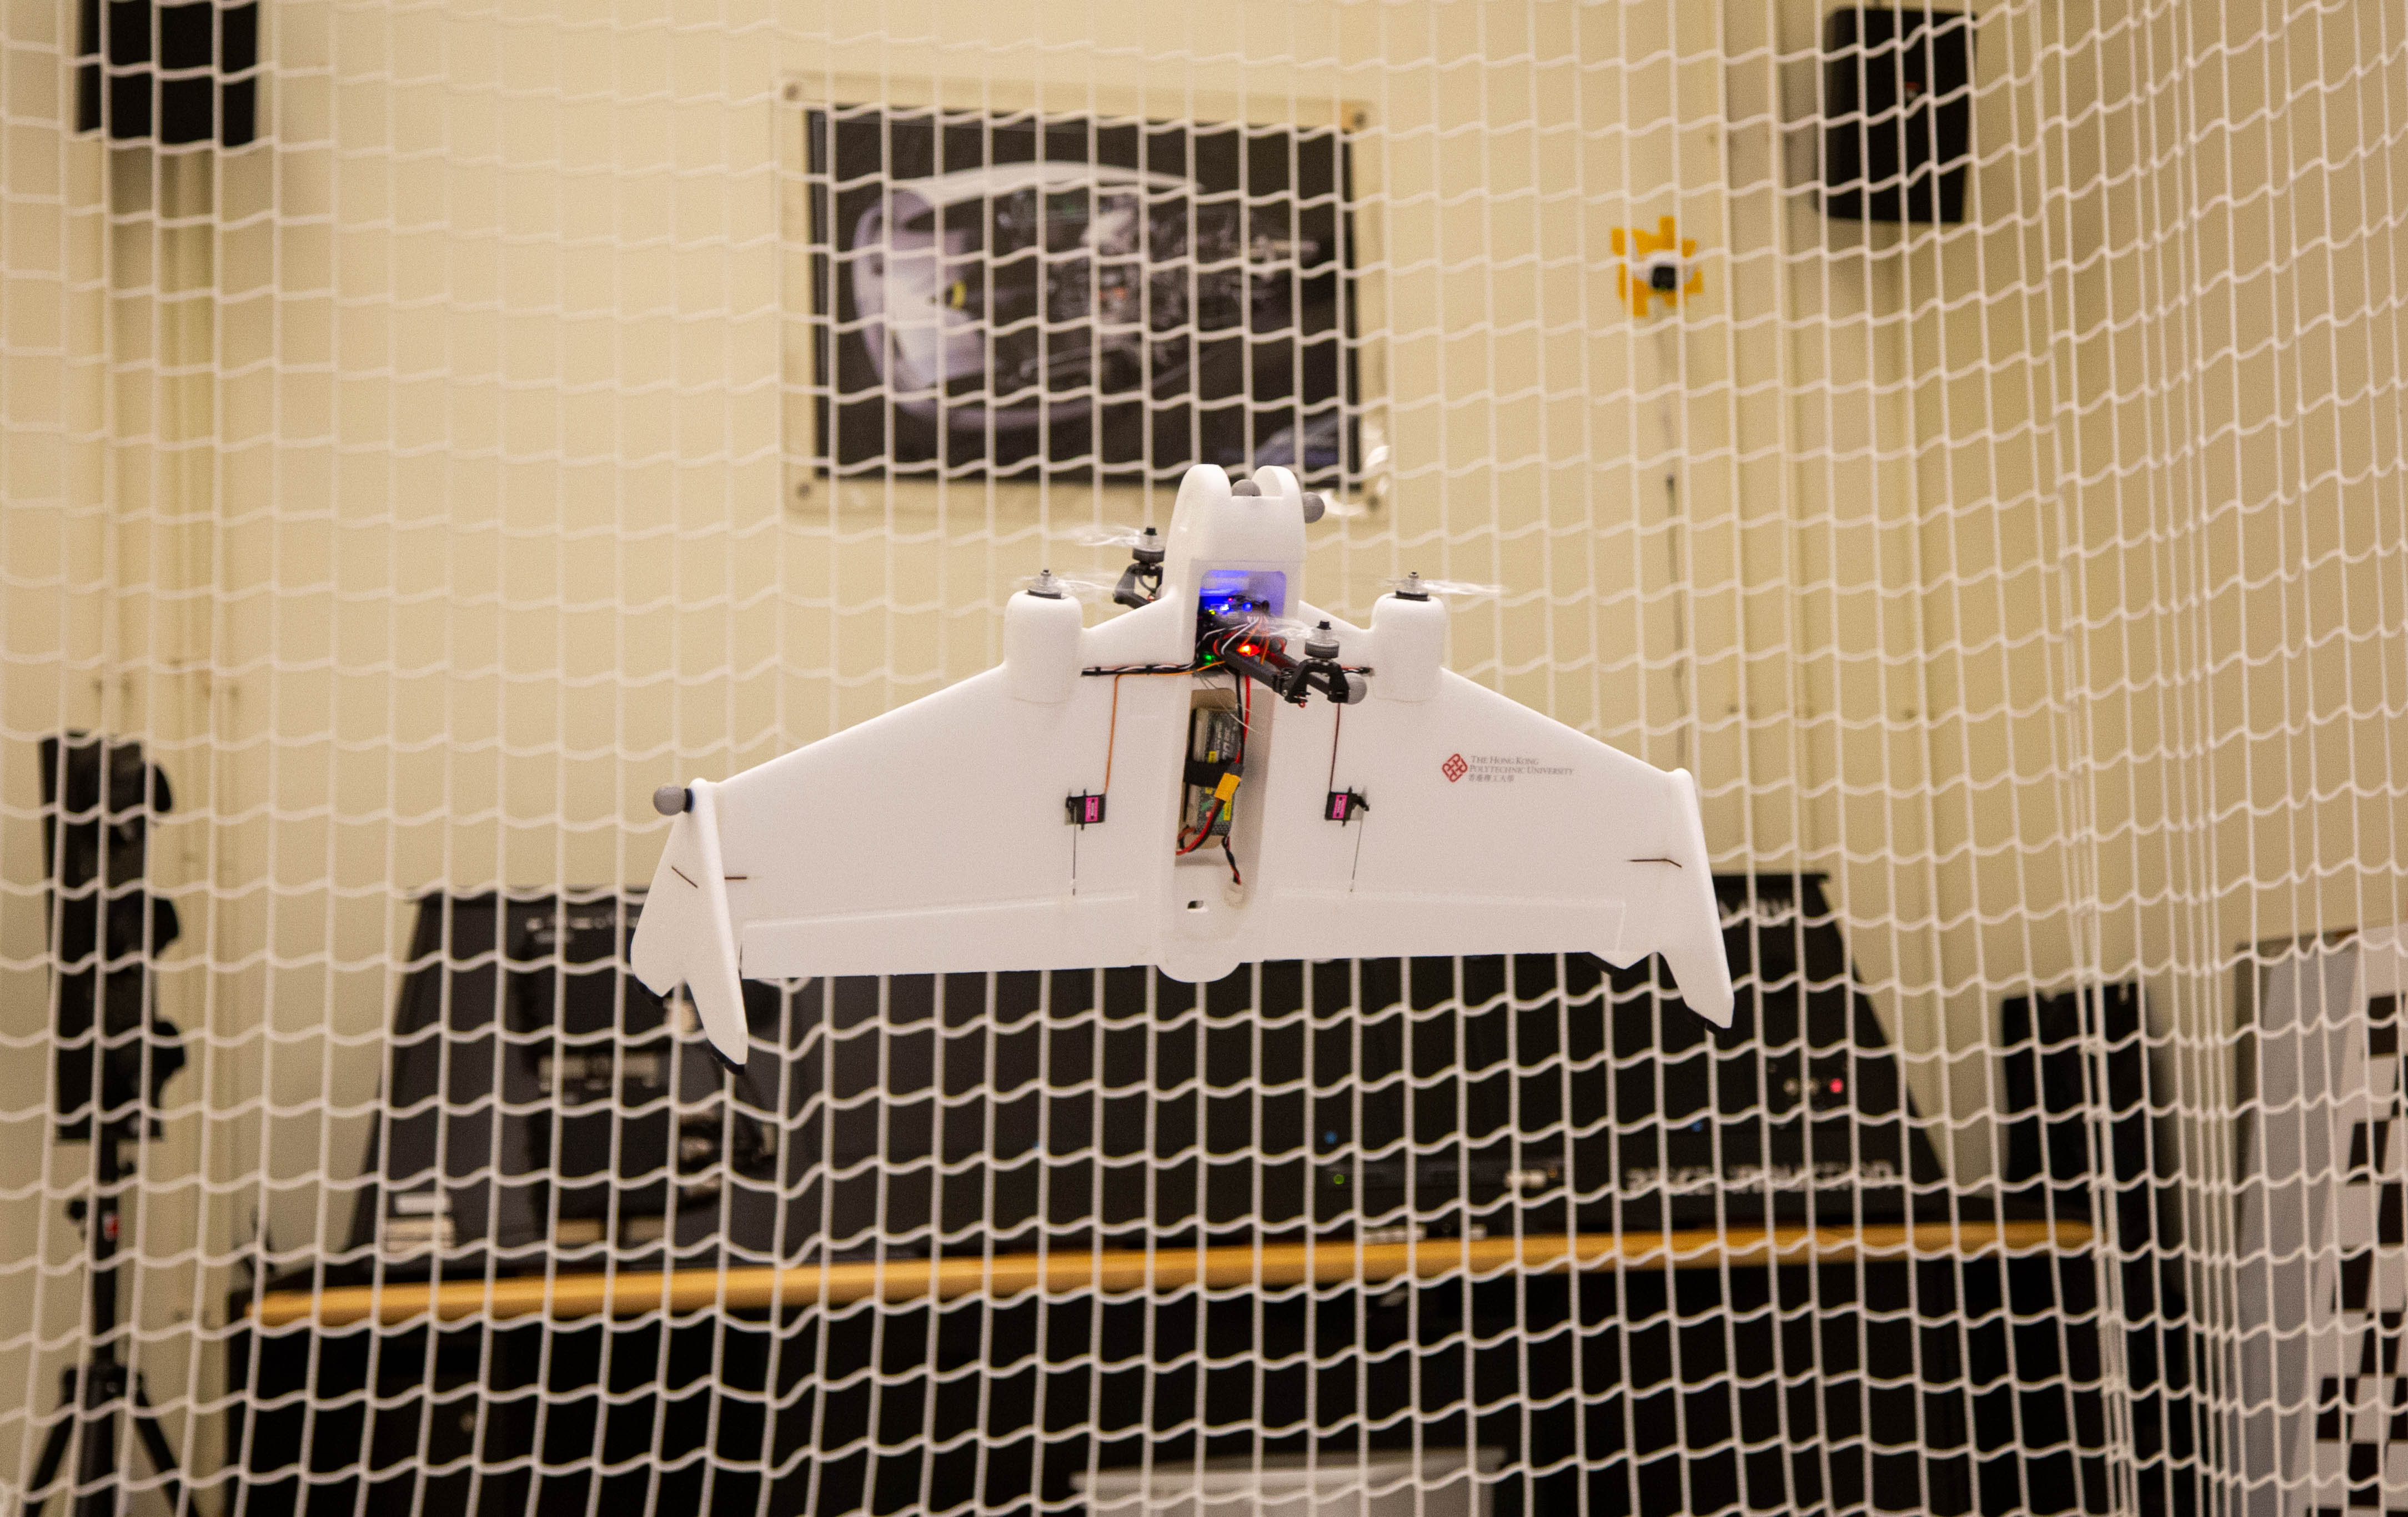
\includegraphics[width=0.7\textwidth]{images/figures/example_figure.jpg}
        \caption{Subfigure b.}
        \label{fig::subfigure_b}
    \end{subfigure}
    \caption{Example subfigures.}
    \label{fig::subfigures}
\end{figure}

You can refer to by subfigures with the corresponding label such as: Figure \ref{fig::subfigure_a} and Figure \ref{fig::subfigure_b}.

All acronyms should be defined in \textit{acronym.tex} and referred to with \textbackslash ac command. The first referred acronym will display the whole name such as \ac{ML}, and only abbreviations will be displayed afterwards such as \ac{ML}.

You can also include url links with url command such as: \url{https://youtube.com}.